%!TEX root = ../thesis.tex
% ******************************* Thesis Appendix B ********************************

% **************************** Define Graphics Path **************************
\ifpdf
    \graphicspath{{Appendix2/Figs/Raster/}{Appendix2/Figs/PDF/}{Appendix2/Figs/}}
\else
    \graphicspath{{Appendix2/Figs/Vector/}{Appendix2/Figs/}}
\fi

\chapter{Directed flow in the Endoplasmic Reticulum} \label{appx:er}
Chapter~\ref{chap:ER} presented evidence for active flow in the endoplasmic reticulum (ER). 
The chapter focussed on work that I had personally contributed to the project; this appendix provides background investigations completed by my collaborators which provide extra context for the work. 
Further details still can be found in \textit{Nature Cell Biology}~\cite{holcman2018single}. 

\section{Flow calculations} \label{appn:flow}
Proteins localised within the ER network, known as luminal proteins, were initially imaged over time using a photoswitchable protein to track their movement. 
Figure~\ref{fig:er-photoconversion} shows a COS-7 cell expressing Dendra2-ER, a green-to-red photoswitchable fluorescent protein which usually has an emission peak at \SI{507}{\nano\metre}. 
After a brief illumination with a \SI{405}{\nano\metre} laser, however, the fluorescent protein is photoconverted and its emission peak shifts to \SI{573}{\nano\metre}. 
This property was exploited to track packets of luminal protein by illuminating a small area of the ER network, then tracking the \SI{573}{\nano\metre} signal, as shown in Figure~\ref{fig:er-photoconversion}. 

\begin{figure}[tbp]
\centering
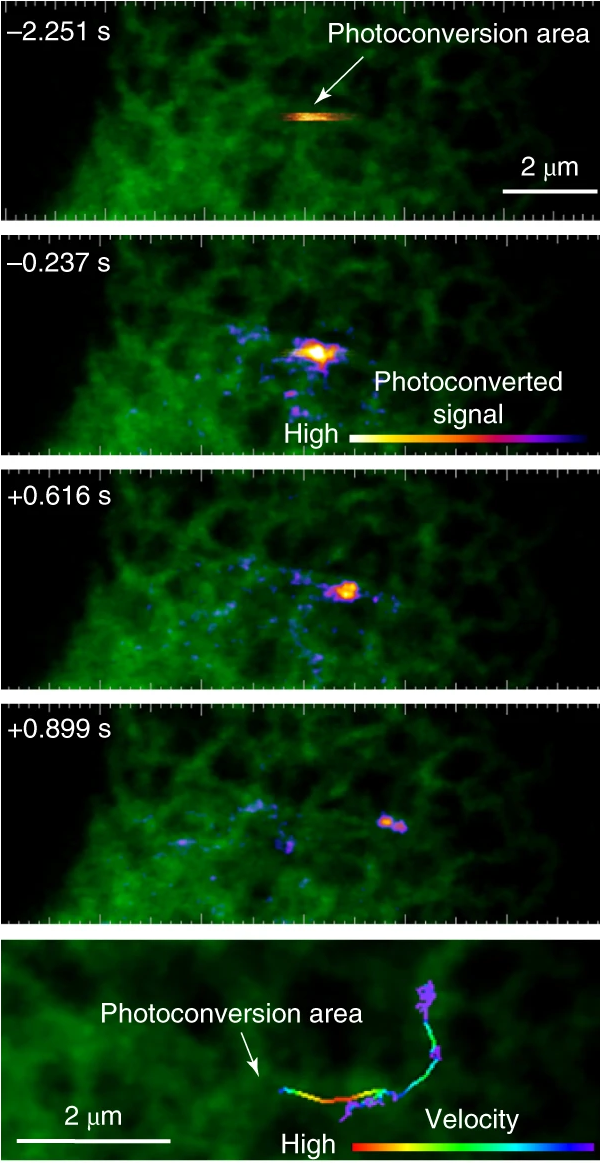
\includegraphics[width=0.65\textwidth]{er-photoconversion}
\caption[Photoconversion allows luminal ER proteins to be tracked]{The figure shows a timelapse of COS-7 labelled with Dendra2-ER, a photoswitchable fluorescent protein. In the first frame, a small area of protein is photoconverted with a \SI{405}{\nano\metre} laser. The converted packet is then tracked, showing fast directed motion as it travels along tubules, but slow Brownian motion at junctions. } 
\label{fig:er-photoconversion}
\end{figure}

From this experiment, it was noted that luminal proteins do not appear to move with exclusively diffusive motion, but rather with directed motion along ER tubes and with Brownian motion at junctions. 
However, the photoswitching experiment can only track one particle group at a time, which is impractical for gathering large numbers of tracks for statistical confidence. 

To gather a large number of luminal protein tracks, Halo-tagged calreticulin (Ctr) was labelled with chloroalkane–tetramethylrhodamine (TMR). 
The brightness and photostability of TMR enabled single particle tracking over long trajectories, with multiple tracks per cell. 
The velocity distributions from the single particle tracking were presented in Figure~\ref{fig:er-directed-flow-velocity}, and show the same velocity distribution as Figure~\ref{fig:er-photoconversion}, with fast motion along tubes and slow, diffusional motion at junctions. 

Two models were created to compare the fit of the data: a purely diffusional model, and a diffusion plus flow model. 
The diffusion model is given by Equation~\ref{eq:diff-model}, where $t$ is a time step, $D$ is the diffusion coefficient, and $\mathbf{\eta}$ is a white noise term. The track data $\mathbf{X}(t)$ and, at a later time point, $\mathbf{X}(t + \Delta t)$ is extracted from the single particle images. 
From this equation the diffusion coefficient is estimated, and the equation is used to produce the solid black line shown in Figure~\ref{fig:er-directed-flow-distribution}. 

\begin{equation} \label{eq:diff-model}
\mathbf{X}(t + \Delta t) = \mathbf{X}(t) + \sqrt{2D\Delta t}\mathbf{\eta}
\end{equation}

The diffusion-only model does not provide a good fit to the data. 
Instead, a model with forced movement as well as a Brownian drift term was used, as shown in Equation~\ref{eq:direct-model}, where $\mathbf{F}$ is a field of force, $\gamma$ is viscosity, and $\mathbf{\dot{\omega}}$ is a noise term derived from thermal agitation.

\begin{equation} \label{eq:direct-model}
\mathbf{\dot{X}} = \frac{\mathbf{F}(\mathbf{X}(t))}{\gamma} + \sqrt{2D}\mathbf{\dot{\omega}}(t)
\end{equation}

Fitting this equation to the single particle tracks produces the dashed line shown in Figure~\ref{fig:er-directed-flow-distribution}. 
This provides a much closer fit to the experimental data, which is particularly noticeable in the cumulative velocity distribution shown in Figure~\ref{fig:er-directed-flow-cumulative}.
In total, \num{80563} single particle tracks were used to calculate model parameters. 

\section{FRET measurements} \label{appn:fret}
When ATP was depleted from cells, a decrease in particle velocity was observed, shown in Figure~\ref{fig:er-atp-depletion}. 
This could either come from a decrease in active transport due to energy starvation, or an increase in the resistance to motion. 
To test the latter hypothesis, a method of measuring ER crowdedness was devised by measuring the fluorescence lifetime (FLT) of a sensitive fluorescence resonance energy transfer (FRET)-based probe. 

The ER-crowdedness FRET probe was based on an expression vector encoding a cytosol-localised crowding probe~\cite{boersma2015sensor}, which was modified to encode an ER-localised probe by amino-terminal addition of mouse preprotrypsin signal sequence and C-terminus addition of a KDEL motif by Gibson assembly. 
SHSY-5Y cells were transfected with the probe, and fluorescent lifetime was measured under a number of treatment conditions, as shown in Figure~\ref{fig:er-fret-flt}.

Under normal conditions, the probe has an average fluorescent lifetime of \SI{2932}{\pico\second}. 
To test the sensitivity of the probe, cells were placed under hyperosmotic or hypo-osmotic conditions with Hanks balanced salt solution (\SI{2.5}{\milli\Molar}, KCl, \SI{1.2}{\milli\Molar} CaCl\textsubscript{2}, \SI{0.5}{\milli\Molar} MgCl\textsubscript{2}, \SI{5}{\milli\Molar} glucose, \SI{10}{\milli\Molar} HEPES pH 7.5) supplemented by \SI{500}{\milli\Molar} NaCl or \SI{0}{\milli\Molar} NaCl respectively. 
Under hyperosmotic conditions, the cell shrinks and we expected luminal crowdedness in the ER to increase; this was measured as a decrease in the fluorescent lifetime, 
to \SI{2546}{\pico\second}. 
Conversely, under hypo-osmotic conditions we expect the cell to expand and crowdedness to decrease, which increased the fluorescent lifetime of the FRET probe to \SI{3302}{\pico\second}. 

When ATP was depleted from the cell, no significant change in fluorescent lifetime was observed compared to the untreated condition. 
This result contradicted the hypothesis that a decrease in particle velocity upon ATP depletion is caused by an increase in resistance from additional crowding, and led us into further investigation of the active process causing ER luminal flow, as detailed in Chapter~\ref{chap:ER}. 

The fluorescent lifetime results are presented as an ER-crowdedness measure in Figure~\ref{fig:er-fret-probe}, where error bars showing standard deviation were calculated from 22 independently sampled cells. 

\begin{figure}[tbp]
\centering
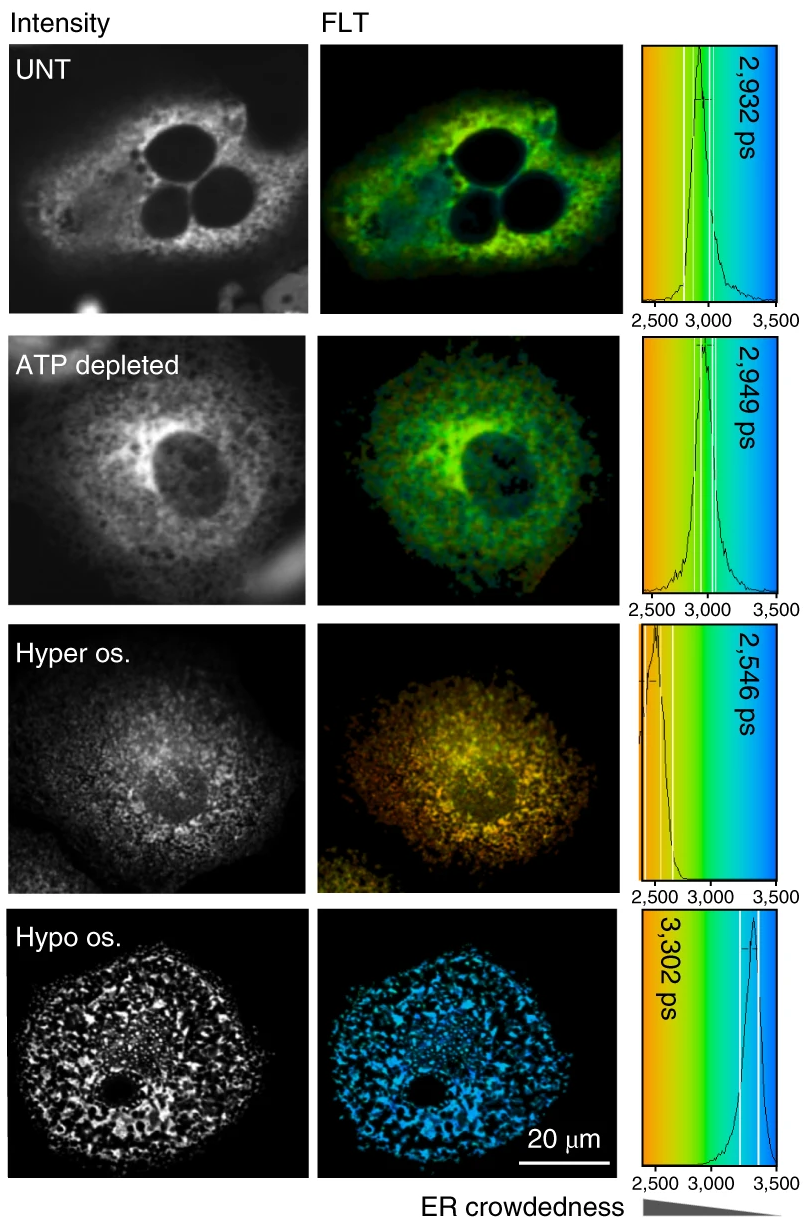
\includegraphics[width=0.85\textwidth]{er-fret-flt}
\caption[Measuring fluorescent lifetime of a FRET-based probe is used to assess ER crowdedness]{Fluorescent lifetime (FLT) was measured in SHSY-5Y cells transfected with a FRET-based probe to assess ER crowdedness. There is no significant difference in FLT between the untreated (UNT) case and the ATP depleted condition. However inducing hyperosmotic or hypo-osmotic conditions with salt solutions causes crowdedness to increase or decrease respectively, leading to measurable changes in the FLT. } 
\label{fig:er-fret-flt}
\end{figure}